\documentclass[../DC2017114Bouma.tex]{subfiles}
\begin{document}
\graphicspath{{03_Contribution/img/}}
\renewcommand{\chaptermark}[1]{\markboth{\thechapter.\ #1}{}}
\renewcommand{\sectionmark}[1]{\markright{#1}{}}

\pagestyle{fancyreport}
\cleartooddpage
\pagestyle{fancyreport}
\chapter{Tracking for Hybrid Systems: Isolated State-and-Input-Triggered Events}\label{ch:order}
In this chapter, an analysis for the behavior of tracking trajectories with isolated state-and-input-triggered jumps of hybrid systems is presented. We will refer to the class of systems as \textit{nonlinear state-and-input-triggered hybrid systems} (NSITHS). The work in this chapter is an extension on \cite{Saccon2014,Rijnen2017}, where a control strategy for \textit{nonlinear state-triggered hybrid systems} (NSTHS) has been presented. In this work, isolated state-and-input-triggered events are considered. This means that the guard functions are activated separately, such that there is always flow between the activations. We will analyze the behavior of the system in the neighborhood of a nominal trajectory assuming that these isolated events also occur in the same sequence locally. However, the timing of the events will differ from the nominal event times for nearby trajectories. The mismatch in event time between the nominal trajectory and state trajectory can result in \textit{peaking behavior} of the tracking error \cite{Menini2001,Biemond2013}. First, we introduce a different notion of error to avoid peaking behavior. After that, a first-order approximation of the NSITHS will be presented in the form of a \textit{linear time-triggered hybrid system} (LTTHS). The chapter extends the work in \cite{Rijnen2017}, which infers stability properties of an NSTHS about a reference trajectory from its corresponding LTTHS. The presumption is made that a similar proof exists for the stability of the LTTHS implying local asymptotic stability of the NSITHS. The realization of this proof is left for future work. Consequentially, conventional stability analysis tools for LTTHS can be used to asses the local stability of te NSITHS. Finally, a short summary of the findings in this chapter is given. The work in this chapter is an extension to \cite{Rijnen2017}, in the sense that the sensitivity analysis in this chapter is suitable for input-dependent guard functions.
\nomenclature[A]{NSITHS}{Nonlinear State-and-Input-Triggered Hybrid System}%
\nomenclature[A]{LTTHS}{Linear Time-Triggered Hybrid System}%

\section{Discontinuous trajectories with state-and-input-triggered jumps}
This section presents \textit{reference-spreading} (RS) for trajectories with isolated events. If the hybrid system starts from a different initial condition than that of the reference trajectory for example, the resulting state trajectory and reference trajectory will likely have non-coinciding event-times. This mismatch in event-times results in peaking behavior in the tracking error when a conventional notion of error in considered. Reference-spreading eliminates peaking behavior by defining the error between two trajectories differently. In order to explain this error notion better, we will first elaborate on the class of systems we consider, on the type of reference trajectories we allow, and we will introduce notation.
\nomenclature[A]{RS}{Reference-Spreading}%

\subsection{Nonlinear state-and-input-triggered hybrid systems}
As presented in Section~\ref{sec:2hyb}, a mechanical system can be described by the hybrid system with impulsive effects framework. Such a system is a nonlinear state-and-input-triggered hybrid system.

\begin{mydef}[NSITHS]\label{def:3nsiths}
A nonlinear state-and-input-triggered hybrid system is a system with dynamics of the form
\begin{align}
\dot{\xb}_j &=\fb_j(\xb_j,\ub_j,t), &\xb_j,\ub_j&\in \mathcal{C}_j\label{eq:3hybimp1}\\
\xb_{j+1} &= \gb_{j+1}(\xb_j,\ub_j,t), &\xb_j,\ub_j&\in \mathcal{D}_{j+1} \label{eq:3hybimp2}
\end{align}
with $\xb_j = \xb(t,j)$ the state, $\ub_j = \ub(t,j)$ the input , $\fb_j$ a nonlinear function, $\mathcal{C}_j$ the flow set after event $j$, and $\mathcal{D}_{j+1}\subseteq\partial \mathcal{C}_j$ a state-input set, where when $\xb_j,\ub_j\in \mathcal{D}_{j+1}$ a state reinitialization is triggered according to $\xb_{j+1} = \gb_{j+1}(\xb_j,\ub_j,t)$.
\end{mydef} 

Consider a nominal trajectory of an NSITHS as illustrated in Figure~\ref{fig:3perturbedtraj} in red. We denote this nominal trajectory $\alphab_j=\alphab(t,j)$ and assume it is the solution to \eqref{eq:3hybimp1},\eqref{eq:3hybimp2} for input signal $\mub_j=\mub(t,j)$ starting from initial condition $\alphab(t_0,0)=\alphab_0\in \mathcal{C}^0$. We moreover pose the following restriction on the nominal trajectory.

\begin{myass}[t-completeness and non-Zeno behavior of $\alphab$]
The reference trajectory $\alphab$ is defined for all $t>t_0$. Also, the reference trajectory segments $\alphab_j$ have non-vanishing time-domains $I^{\alphab}_j=[\tau_j,\tau_{j+1}]$, where $\tau_j$ is the $j^{\textnormal{th}}$ event time.\label{ass:nonzeno}
\end{myass}

Assumption~\ref{ass:nonzeno} guarantees that the number of events $N$ will only go to infinity if time $t$ goes to infinity as well. This assumption is often made in analysis using hybrid systems. It can be guaranteed that there is non-zero time between events, if $\gb_{j+1}(\alphab_j(\tau_{j+1}),\mub_j(\tau_{j+1}))\notin \mathcal{D}_{j+1}$ for all $j\in\{0,1,\dots,N\}$.

Consider now a state trajectory $\xb$ starting from initial condition $\xb(t_0,0)=\xb_0(\epsilon)=\alphab_0+\epsilon \zb_0$ different than that of the reference trajectory $\alphab$ and with input $\ub_j(\epsilon)=\mub_j+\epsilon \vb_j$. In this $\zb_0 = \frac{\partial\xb_0}{\partial\epsilon}$, $\mub_j = \mub(t,j)$ the feedforward corresponding to $\alphab_j$, and $\vb_j = \vb(t,j)$ the feedback. An example of a trajectory $\xb$ is shown in Figure~\ref{fig:3perturbedtraj}.

\nomenclature[G]{$\epsilon$}{The scalar perturbation parameter}%
\nomenclature[S]{$(\cdot)_{\epsilon}$}{A variable dependent on the initial perturbation}%
\begin{figure}[h]
\centering
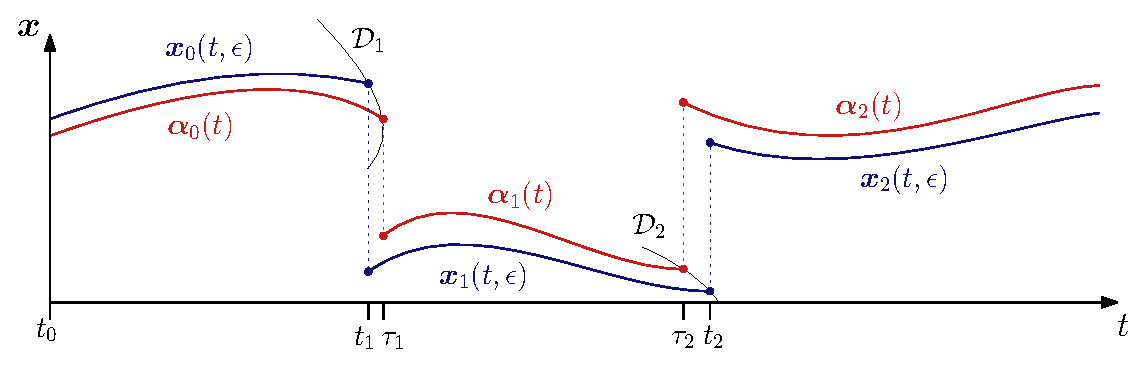
\includegraphics[width=.9\textwidth]{perturbedtraj.eps}\caption{A nominal (red) and a perturbed (blue) trajectory of a hybrid system with impulsive effects are depicted in this figure. Due to the perturbation in the blue trajectory, a mismatch between the perturbed and the nominal event times arises.} \label{fig:3perturbedtraj}
\end{figure}

For the nominal trajectory the state and input are known over the entire time-domain, meaning that the event-times are also known. For the perturbed trajectory this is not the case. There will be a mismatch between the nominal event times $\tau_1$, $\tau_2$ and the perturbed event times $t_1$, $t_2$. Now we take a closer look at the first event of Figure~\ref{fig:3peakerror}, to illustrate the peaking behavior as a result of a jump mismatch. In Figure~\ref{fig:3peakerror}, the state evolution $\xb$ of the first event is depicted besides the conventional tracking error $||\xb-\alphab||$ where both trajectories are considered a function of conventional time $t$ alone. One can clearly see that a peak arises in the tracking error when the jump times do not coincide. At $t_1$ the state trajectory jumps, while the reference trajectory does not. At $\tau_1$ the reference trajectory jumps as well. This means that in $[t_1,\tau_1]$, a post-event state trajectory is compared to a ante-event reference trajectory, resulting in a large peak in the tracking error. This is undesirable in stability analysis and may for example lead to large and unnecessary actuation forces when considered in feedback control.

\begin{figure}[h]
\centering
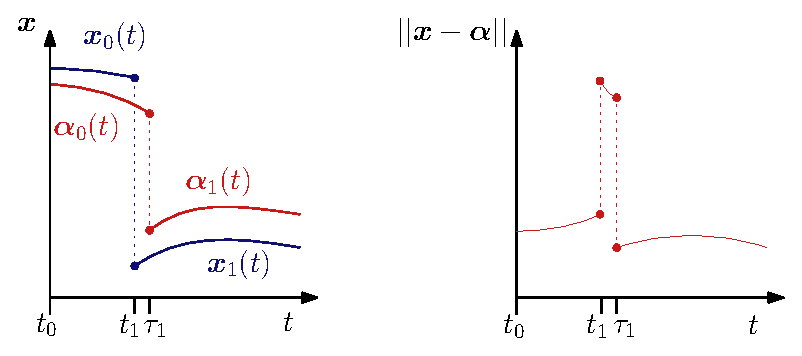
\includegraphics[width=.66\textwidth]{peakerror.eps}\caption{A closer look at the first event of the trajectory in Figure~\ref{fig:3perturbedtraj}. On the left the state-evolution $\xb$ is depicted and on the right the tracking error $||\xb-\alphab||$. A clear peak can be noticed in the tracking error as a result from the event-time mismatch.} \label{fig:3peakerror}
\end{figure}

In the next section, a different notion of error will be introduced that does not illustrate peaking behavior.
\nomenclature[G]{$\Delta$}{The linearization of the perturbed event time around zero perturbation}%
\nomenclature[R]{$o(\cdot)$}{Little-o notation}%
\nomenclature[R]{$\Gb$}{Positively homogeneous jump gain for the perturbed state direction}%
\nomenclature[R]{$\Jb$}{Positively homogeneous jump gain for the perturbed input direction}%
\nomenclature[R]{$D_i(\cdot)$}{The derivative with respect to the $i$th term}%

\subsection{Reference-spreading}
To avoid peaking behavior in the tracking error, in \cite{Saccon2014} a novel notion of error is presented which is named reference spreading in \cite{Rijnen2016}. This control strategy uses reference trajectories which are extended beyond event-times, such that an ante-event state trajectory can always be compared to an ante-event reference trajectory and a post-event state trajectory can always be compared to a post-event reference trajectory. This is illustrated in Figure~\ref{fig:3refspread}, where the reference trajectory $\alphab_j$ is extended resulting in $\bar{\alphab}_j$. The extension is made by forward integrating the vector field $\fb_j$ beyond $\tau_{j+1}$ and backward integrating $\fb_j$ before $\tau_j$, for all $j\in\{0,1,\dots,N\}$. Adopting the notation of \cite{Goebel2009}, the hybrid domain of $\alphab$ is defined by segments $I_j^{\alphab} = [\tau_j,\tau_{j+1}]$, which together form the entire domain of $\alphab$ as
\begin{align}
\dom\alphab = \bigcup^N_{j=0}I^{\alphab}_j\times\{j\}.
\end{align}
\nomenclature[R]{$I$}{Domain of a segment}%
Similarly the state segments $\xb_j$ are defined on the time intervals $I_j^\xb = [t_j,t_{j+1}]$ with the entire domain defined as
\begin{align}
\dom\xb = \bigcup^N_{j=0}I^{\xb}_j\times\{j\}.
\end{align}
The domain of the extended reference trajectory segments is extended such that $I^{\xb}_j\subseteq I^{\bar{\alphab}}_j$. The set of jump times of $\alphab_j$ and $\xb_j(\epsilon)$ are denoted as
\begin{align}
\text{eve}\ \alphab &= \bigcup_{j=1}^N \{\tau_j\}\times\{j-1\},\\
\text{eve}\ \xb &= \bigcup_{j=1}^N \{t_j\}\times\{j-1\},
\end{align}
respectively.
\begin{figure}[h]
\centering
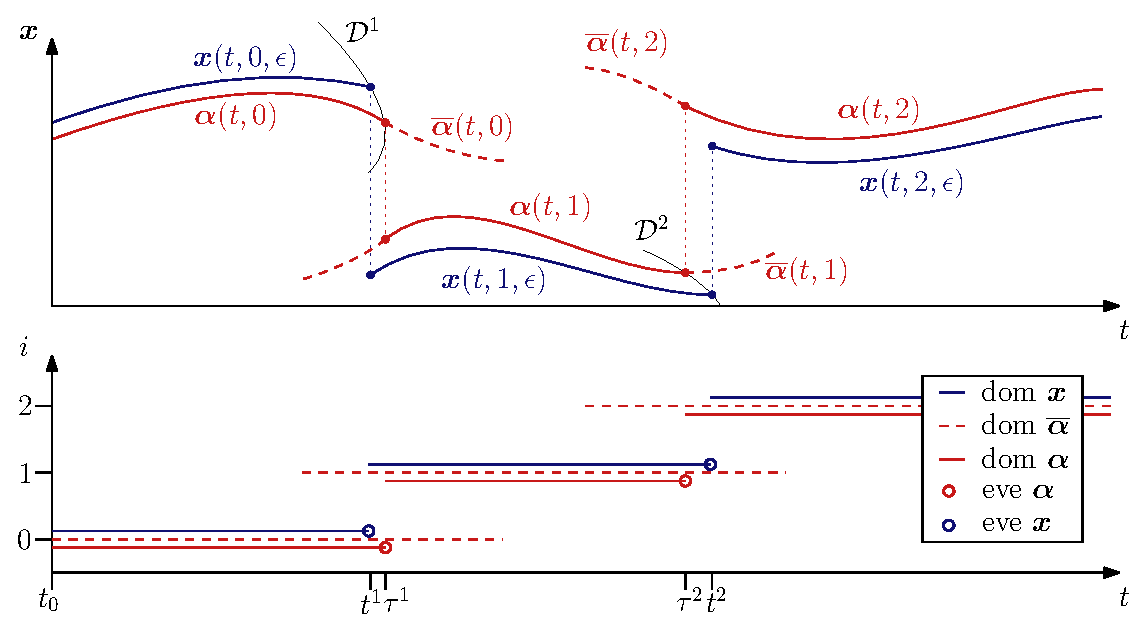
\includegraphics[width=.9\textwidth]{refspreaddom.eps}\caption{An illustration of the nominal reference trajectory (red) and the perturbed trajectory (blue), where the nominal reference trajectory is extended such that $\dom \xb\subseteq\dom \bar{\alphab}$.} \label{fig:3refspread}
\end{figure}

Now a continuity based assumption on the vector field $\fb_j$ is defined. This assumption (along with other assumptions) is necessary to make sure that the ante-event state of the perturbed trajectory $\xb_j(t_{j+1},\epsilon)$ lies close to the ante-event state of the nominal trajectory $\alphab_j(\tau_{j+1})$, which is necessary to define an approximation of the perturbed trajectory.

\begin{myass}[Lipschitz continuity of $\fb$]\label{ass:lipschitz}
We assume that in a neighborhood of the reference trajectory $\alphab$, $\fb$ is Lipschitz with respect to $\xb$ uniformly in $t$ and $j$. I.e., $\exists\varepsilon_{\fb}>0$ and $\exists L$, independent of $t,j$, such that $\forall j$, $||\fb_j(\ab,t) - \fb_j(\bb,t)||<L||a-b||$, $\forall t\in (\tau_j - \varepsilon_{\fb},\tau_{j+1} + \varepsilon_{\fb})$ and $\forall \ab,\bb\in B_{\varepsilon_{\fb}}(\bar{\alphab}_j)$, where $B_{\varepsilon_{\fb}}(\bar{\alphab}_j)$ is a ball with radius $\epsilon_{\fb}$ around $\bar{\alphab}_j)$.
\end{myass}

In the lower plot of Figure~\ref{fig:3refspread}, the hybrid time domains of $\xb$, $\alphab$ and $\bar{\alphab}$ are illustrated. Note that for every $j$, it holds that $I^{\xb}_j\subseteq I^{\bar{\alphab}}_j$. This means that the tracking error $||\xb-\bar{\alphab}||$ is continuous for fixed $j$, even in the case where $t_j\neq\tau_j$. Using this notion of error leaves only one jump in the tracking error, even under the presence of event-time mismatches. More importantly, the peak in the tracking error is avoided, an ante-event state trajectory will not be compared to a post-event reference trajectory (and vice versa) anymore. This is illustrated in Figure~\ref{fig:3refspreaderrors}, where the tracking errors with and without reference spreading are compared.

\begin{figure}[h]
\centering
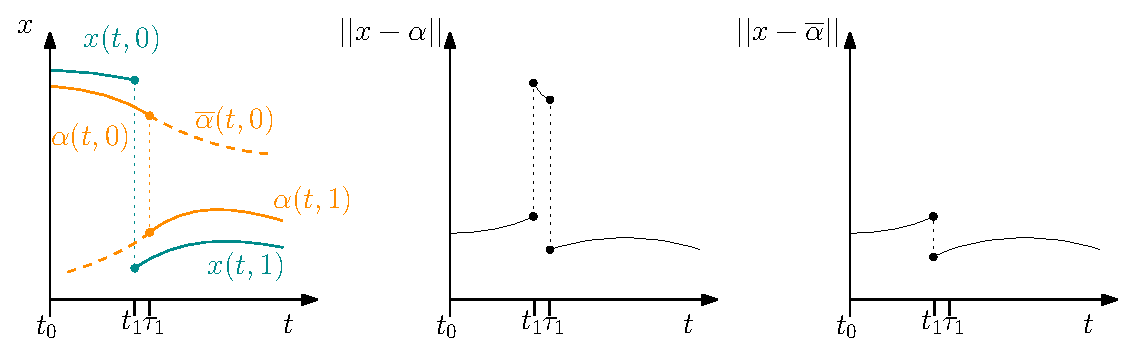
\includegraphics[width=\textwidth]{refspreaderrors.eps}\caption{A close up of the  first event of the reference trajectory, in which the peaking behavior is cleary removed by evaluating the extended reference trajectory.} \label{fig:3refspreaderrors}
\end{figure}

In the next section, the error defined using reference spreading will be used to construct a first-order approximation of perturbed trajectories with isolated events.

\section{First-order approximation of trajectories with ordered guard-activations}\label{sec:3approx}
In \cite{Khalil1996} a sensitivity analysis is presented, where so-called sensitivity functions are used to provide first-order approximations of the effects of parameter variations on solutions. These sensitivity functions can also be used to approximate the solution under sufficiently small parameter variations. For the class of systems we consider here, the sensitivity equations describe the system's response to perturbations in initial condition and input. These perturbation dynamics can be used to formulate a first-order approximation of the perturbed state of the system. To find a first-order approximation of state reinitializations in nonsmooth trajectories, an extension to this sensitivity analysis is necessary in the form of a linearized jump gain. The linearized jump gain and the linearized perturbation dynamics together define the LTTHS. In \cite{Rijnen2017} stability properties of an NSTHS are associated with the stability the corresponding LTTHS. In this section the LTTHS is derived for an NSITHS, which can be used to assess the stability of the NSITHS under the presumption that a similar relation between the LTTHS and NSITHS exists. The proof for this relation is left for future work. For a more thorough derivation of the analysis that follows, Appendix~\ref{app:Csensitivity} should be consulted. We will first pose few assumptions on the reference events and jump maps that are required for the sensitivity analysis. First, we assume transversality of the reference events for which we assume the existence of a guard function that locally describes the flow and jump sets about each reference event.

\begin{myass}[Existence of a guard function]\label{ass:existence}
We assume that there exist constants $\varepsilon_\gamma$, and real valued guard function $\gamma(\xb,\ub,t,j)$ which is continuously differentiable with respect to $\xb$, $\ub$, and $t$, for each $j\in \{1,2,...,N\}$, such that
\begin{equation}
\begin{array}{llll}
\gamma_{j+1}(\xb_j,\ub_j,t) > 0 & &	&(\xb,\ub) \in B_{\varepsilon_\gamma}(\alphab_j(\tau),\mub_j(\tau))\cap \mathcal{C}_j\setminus\partial \mathcal{C}_j\\
\gamma_{j+1}(\xb_j,\ub_j,t) = 0 & &	&(\xb,\ub) \in B_{\varepsilon_\gamma}(\alphab_j(\tau),\mub_j(\tau))\cap \mathcal{D}_{j+1}\\
\gamma_{j+1}(\xb_j,\ub_j,t) < 0 & &	&(\xb,\ub) \in B_{\varepsilon_\gamma}(\alphab_j(\tau),\mub_j(\tau))\cap (\Rbb^n \times \Rbb^m \times \Rbb)\setminus \mathcal{C}_j
\end{array}
\end{equation}
where $B_{\varepsilon_\gamma}(\alphab_j(\tau),\mub_j(\tau))$ is a ball with radius $\varepsilon_{\gamma}$ around $\alphab_j(\tau),\mub_j(\tau)$ with $\tau = \tau_{j+1}$. $\mathcal{C}_j$ is the flow set of a trajectory after event $j$ and $\mathcal{D}_{j+1}\subseteq\partial \mathcal{C}_j$ is the event set which triggers event $j+1$, where $\partial \mathcal{C}_j$ represents the boundary of flow set $\mathcal{C}_j$.
\end{myass}

\begin{myass}[Transversal guard activations]\label{ass:transversality}
Under Assumption~\ref{ass:existence}, we assume there exists a constant $c>0$, such that
\begin{equation}
D_1\gamma_j(\alphab_j,\mub_j,t)\cdot\fb_j(\alphab_j,\mub_j,t) + D_2\gamma_j(\alphab_j,\mub_j,t)\cdot\fb_j(\alphab_j,\mub_j,t) + D_3\gamma_j(\alphab_j,\mub_j,t) \leq -c,
\end{equation}
for every event time $(t,j) \in \eve \alphab$.
\end{myass}

\begin{myremark}
The time derivative of the guard function $\gamma^{\text{sl}\rightarrow\text{st}} = \sqrt{\zetab_t^T\zetab_t}$, is undefined when $\gamma^{\text{sl}\rightarrow\text{st}} = 0$. Therefore, a Taylor expansion is used to find the left limit of $\dot{\gamma}^{\text{sl}\rightarrow\text{st}}$ at $t = \tau_j$, to check whether the guard is activated transversally. More information on this can be found in Appendix~\ref{app:hybriddisc}.
\end{myremark}

%\begin{myass}[Isolated events]\label{ass:guardeventpair}
%With the set of all participating guard functions $\gamma^{\textnormal{part}}$, we assume that there exist a constant $\varepsilon_\gamma$, and set of nominal activated guard functions $\gamma^{\textnormal{nom}}_j$, such that
%\begin{align}
%\gamma^{\textnormal{part}}\setminus\gamma^{\textnormal{nom}}_j > 0,\quad \forall \xb,\ub\in B_{\varepsilon_\gamma}(\alphab(\tau,j),\mub(\tau,j),\tau),
%\end{align}
%where $\gamma_j = \gamma(\xb,\ub,t,j)$, and $B_{\varepsilon_\gamma}(\alphab(\tau,j),\mub(\tau,j),\tau)$ is a ball with radius $\varepsilon_{\gamma}$ centered around the ante-event state and input $\alphab(\tau,j),\mub(\tau,j)$ of event $j$.
%\end{myass}

%Assumption~\ref{ass:guardeventpair} makes sure that the perturbed trajectory will activate the same guard functions as the reference trajectory.
$\gamma_j(\xb_j,\ub_j,t) = 0$ represents the set where an event will happen, which together with Assumption~\ref{ass:transversality} guarantees that an event will happen, even under perturbations. Assumption~\ref{ass:transversality} assumes that the vector field pushes the reference trajectory out of the flow set $\mathcal{C}_j$, and that grazing incidents are avoided. The combination of the existence of a guard function in an area around the nominal ante-event state and the transversal guard activation guarantees that there exists a range of perturbations where the guard is activated as well. Now an assumption on the jump map $\gb$ is posed.

\begin{myass}[Locally differentiability of jump maps]\label{ass:jump}
We assume that for all $j \in [0,1,2,...,N]$ the jump map $\gb_{j+1}(\xb_j,\ub_j)$ is locally differentiable, in the sense that $D_1\gb_{j+1}(\xb_j,\ub_j)$ and $D_2\gb_{j+1}(\xb_j,\ub_j)$ exist in the ball $B_{\varepsilon_{\gamma}}(\alphab_j(\tau),\mub_j(\tau),\tau)$, where $\tau = \tau_{j+1}$.
\end{myass}

The differentiability of the jump map is necessary to construct a first-order approximation of the perturbed state trajectory. This will be explained in more detail in the next section.

\subsection{Sensitivity analysis}
The sensitivity analysis for the continuous segments of a perturbed trajectory, gives a set of equations which describe the system's reaction to an initial state-and-input perturbation. The state-and-input perturbation represents a modeling error. A continuous segment of the perturbed state is given by
\begin{align}
\xb_j(t,\epsilon) = \xb_j(t_j,\epsilon) + \int_{t_j}^{t_{j+1}}\fb_j(\xb_j(s,\epsilon),\ub_j(s,\epsilon),s)ds.\label{eq:3xpert}
\end{align}
To find a first-order approximation of the perturbed state, the perturbed state direction $\zb(t)$ and the perturbed input direction $\vb(t)$ are defined as
\begin{align}
\zb_j = \left.\frac{\partial\xb_j(\epsilon)}{\partial\epsilon}\right|_{\epsilon=0},\text{ and } \vb_j = \left.\frac{\partial\ub_j(\epsilon)}{\partial\epsilon}\right|_{\epsilon=0},
\end{align}
with $\zb_j(t) = \zb(t,j)$, and $\vb_j(t) = \vb(t,j)$. It follows that, conforming to the sensitivity analysis presented in \cite{Khalil1996},
\begin{align}
\xb_j(\epsilon) &= \xb_j(0) + \epsilon\left.\frac{\partial\xb_j(\epsilon)}{\partial\epsilon}\right|_{\epsilon=0} + o(\epsilon),\label{eq:3taylor}\\
&= \bar{\alphab}_j + \epsilon\bar{\zb}_j + o(\epsilon),
\end{align}
with $o(\epsilon)$ indicating the little-o notation of $\epsilon$ which represents higher order terms. To find a first order approximation of the $\dot{\xb}_j(\epsilon)$, an expression for $\dot{\zb}_j$ should be found. By first taking the partial derivative with respect to $\epsilon$ and then with respect to $t$ of $\eqref{eq:3xpert}$, the perturbation dynamics are found to be
\begin{align}
\dot{\zb}_j = \Ab_j(t)\zb_j +\Bb_j(t)\vb_j,\label{eq:3zdot}
\end{align}
with
\begin{align}
\Ab_j(t) &= D_1\fb_j(\alphab_j,\mub_j,t),\\
\Bb_j(t) &= D_2\fb_j(\alphab_j,\mub_j,t),
\end{align}
where $D_a$ represents the partial derivative with respect to the $a^{\text{th}}$ argument. The first order approximation of the perturbed state dynamics in continuous time is then defined as
\begin{align}
\dot{\xb}_j(\epsilon) \approx \dot{\alphab}_j + \epsilon\dot{\zb}_j,
\end{align}
where $\dot{\alphab}_j$ is known and $\dot{\zb}_j$ is given by \eqref{eq:3zdot}. Now the first-order approximation is defined for the continuous segments of a trajectory. What remains is that the state reinitializations should be linearized as well. The reinitialization of the nominal trajectory satisfies
\begin{align}
\alphab_{j+1}(\tau_{j+1}) = \gb_{j+1}(\alphab_j(\tau_{j+1}),\mub_j(\tau_{j+1}),\tau_{j+1}),\label{eq:3g}
\end{align}
and the reinitialization of the perturbed state is described by
\begin{align}
\xb_{j+1}(t_{j+1},\epsilon) = \gb_{j+1}(\xb_j(t_{j+1},\epsilon),\ub_j(t_{j+1},\epsilon),t_{j+1}).
\end{align}
Similar to the Taylor expansion used in \eqref{eq:3taylor}, the state and input of the next segment evaluated at the perturbed event time $t_{j}$ can be expanded to
\begin{align}
\xb_j(t_{j},\epsilon) &= \bar{\alphab}_j(t_{j}) + \epsilon\bar{\zb}_j(t_{j}) + o(\epsilon),\label{eq:3xexpand}\\
\ub_j(t_{j},\epsilon) &= \bar{\mub}_j(t_{j}) + \epsilon\bar{\vb}_j(t_{j}) + o(\epsilon).\label{eq:3uexpand}
\end{align}
The same can be done for $\alphab_j(t_{j})$, $\mub_j(t_{j})$, $\zb_j(t_{j})$, and $\vb_j(t_{j})$, which when substituted in \eqref{eq:3xexpand} and \eqref{eq:3uexpand} results in
\begin{align}
\xb_j(t_{j},\epsilon) &= \alphab_j(\tau_j) + \epsilon\dot{\alphab}_j(\tau_j)\Delta_j + \epsilon\zb_j(\tau_j) + o(\epsilon),\label{eq:3xexpand2}\\
\ub_j(t_{j},\epsilon) &= \mub_j(\tau_j) + \epsilon\dot{\mub}_j(\tau_j)\Delta_j + \epsilon\vb_j(\tau_j) + o(\epsilon),\label{eq:3uexpand2}
\end{align}
with
\begin{align}
\Delta_{j} = \left.\frac{\partial t_{j}}{\partial\epsilon}\right|_{\epsilon=0}.\label{eq:3Delta}
\end{align}
To find $\Delta_{j}$, we observe that
\begin{align}
\gamma_j(\xb_{j-1}(t_{j},\epsilon),\ub_{j-1}(t_{j},\epsilon),t_{j}) = 0.\label{eq:3gamma}
\end{align}
Note that $\gamma_j$ is dependent on the input $\ub_j$, whereas in \cite{Chen2018a} the sensitivity analysis is performed for guard functions which solely depend on state $\xb_j$ and time $t$. From \eqref{eq:3gamma} the expression for $\Delta_{j}$ is found to be
\begin{align}
\Delta_{j} = -\frac{D_1\gamma^{-}\cdot\zb^- + D_2\gamma^{-}\cdot\vb^-}{\dot{\gamma}^{-}},\label{eq}
\end{align}
with
\begin{align*}
\gamma^- &= \gamma_j(\alphab_{j-1}(\tau_j),\mub_{j-1}(\tau_j),\tau_j),\\
\dot{\gamma}^- &= D_1\gamma^-\cdot\dot{\alphab}_{j-1}(\tau_j) + D_2\gamma^-\cdot\dot{\mub}_{j-1}(\tau_j) + D_3\gamma^-,\\
\zb^- &= \zb_{j-1}(\tau_j),\\
\vb^- &= \vb_{j-1}(\tau_j),
\end{align*}
where the $-$ superscript indicates a left limit of event $j$. Expanding \eqref{eq:3g} and substituting the result into \eqref{eq:3xexpand2} gives
\begin{equation}
\zb^+ = D_1\gb^-\cdot\left(\zb^- + \dot{\alphab}^-\Delta_j\right) + D_2\gb^-\cdot\left(\vb^- + \dot{\mub}^-\Delta_j\right) + D_3\gb^-\cdot\Delta_j - \dot{\alphab}^+\Delta_j,
\end{equation}
with
\begin{align*}
\gb^- &= \gb_j(\alphab^-,\mub^-,\tau_j),\\
\zb^+ &= \zb_j(\tau_j),\\
\alphab^- &= \alphab_{j-1}(\tau_j),\\
\alphab^+ &= \alphab_j(\tau_j),\\
\mub^- &= \mub_{j-1}(\tau_j).
\end{align*}
Here the $+$ superscript indicates the right limit of event $j$. This can finally be rewritten to
\begin{align}
\zb^+ = \Lb_j(\tau_j)\begin{bmatrix}
\zb^- \\ \vb^-
\end{bmatrix},
\end{align}
with 
\begin{align*}
\Lb_j(\tau_j) &= \begin{bmatrix}
\Gb_j(\tau_j) & \Jb_j(\tau_j)
\end{bmatrix},\\
\Gb_j(\tau_j) & = D_1\gb^- - \left(\dot{\gb}^- - \fb^+\right)\frac{D_1\gamma^-}{\dot{\gamma}^-},\\
\Jb_j(\tau_j) & = D_2\gb^- - \left(\dot{\gb}^- - \fb^+\right)\frac{D_2\gamma^-}{\dot{\gamma}^-},
\end{align*}
where
\begin{align*}
\fb^- &= \fb_{j-1}(\alphab_{j-1}(\tau_j),\mub_{j-1}(\tau_j),\tau_j),\\
\fb^+ &= \fb_j(\alphab_j(\tau_j),\mub_j(\tau_j),\tau_j),\\
\dot{\gb}^- &= D_1\gb^-\cdot \fb^- + D_2\gb^-\cdot \dot{\mub}^- + D_3\gb^-.
\end{align*}

\subsection{Linear time-triggered hybrid system}
The sensitivity analysis performed in the previous section will be used next to define the LTTHS associated to reference trajectory $\alphab$ and the NSITHS defined in Definition~\ref{def:3nsiths}. The LTTHS converts the state-triggered behavior of the NSITHS to a time-triggered behavior using a first order approximation of the state jumps. Where the jump times of the NSITHS are unknown, the LTTHS jumps at the same event-times as the nominal trajectory $\alphab$. In \cite{Rijnen2017}, a proof is given that stability of the LTTHS implies local asymptotic stability of a NSTHS. Although not fully proven, we expect that that result carries over to the implication that uniform asymptotic stability of the LTTHS implies local asymptotic stability of the NSITHS. Since the stability assessment of LTTHS is well established in literature, the LTTHS can then be used to conveniently assess the local asymptotic stability of the NSITHS. Now the LTTHS is formally defined.

\begin{mydef}[LTTHS]\label{def:3ltths}
The linear time-triggered hybrid system associated with the reference trajectory $\alphab$ and the NSITHS \eqref{eq:3hybimp1},\eqref{eq:3hybimp2} is given by
\begin{align}
\dot{\zb}_j &= \Ab_j(t)\zb_j + \Bb_j(t)\vb_j &(t,j)&\in \dom\ \alphab\\
\zb^+ &= \Lb_{j+1}(t) \begin{bmatrix}\zb^- \\ \vb^-\end{bmatrix} &(t,j)&\in \eve\ \alphab
\end{align}
with initial condition $\zb(t_0,0)=z_0$, $\zb^+ = \zb(\tau_j,j)$, $\zb^- = \zb(\tau_j,j-1)$,
\begin{align*}
\Ab_j(t) &= D_1\fb_j(\alphab_j(t),\mub_j(t),t)\\
\Bb_j(t) &= D_2\fb_j(\alphab_j(t),\mub_j(t),t)\\
\Lb_j &= \begin{bmatrix}\Gb_j(t) & \Jb_j(t)\end{bmatrix},\\
\Gb_j &= D_1\gb^- - \left(\dot{\gb}^- - \fb^+\right)\frac{D_1\gamma^-}{\dot{\gamma}^-},\\
\Jb_j &= D_2\gb^- - \left(\dot{\gb}^- - \fb^+\right)\frac{D_2\gamma^-}{\dot{\gamma}^-},
\end{align*}
and
\begin{align*}
\fb^- &= \fb_{j-1}(\alphab_{j-1}(\tau_j),\mub_{j-1}(\tau_j),\tau_j),\\
\fb^+ &= \fb_j(\alphab_j(\tau_j),\mub_j(\tau_j),\tau_j),\\
\gb^- &= \gb_{j}(\alphab_{j-1}(\tau_j),\mub_{j-1}(\tau_j),\tau_j),\\
\dot{\gb}^- &= D_1\gb^-\cdot \fb^- + D_2\gb^-\cdot \dot{\mub}^- + D_3\gb^-,\\
\gamma^- &= \gamma_j(\alphab_{j-1}(\tau_j),\mub_{j-1}(\tau_j),\tau_j),\\
\dot{\gamma}^- &= D_1\gamma^-\cdot\dot{\alphab}_{j-1}(\tau_j) + D_2\gamma^-\cdot\dot{\mub}_{j-1}(\tau_j) + D_3\gamma^-.
\end{align*}
\end{mydef}
The LTTHS defined in Definition~\ref{def:3ltths} gives a first order approximation of the NSITHS about the state-input reference trajectory $(\alphab,\mub)$. With a nominal trajectory $\alphab$ with input $\mub$, the perturbed trajectory $\xb_j(\epsilon)$ is the trajectory starting from initial condition $\xb_0(\epsilon) = \alphab_0 + \epsilon\zb_0$ and with input $\ub_j(\epsilon) = \mub_j + \epsilon\vb_j$. The first order approximation is then defined as $\xb_j(\epsilon) \approx \bar{\alphab}_j + \epsilon\bar{\zb}_j$, with $\zb$ defined by the LTTHS. The reader should be aware that the term $\vb^-$ is not an input that can be freely chosen. $\vb^-$ is directly related to $\vb_j$, as it is a result of the feedback law implemented during the continuous segment before the event. Also, note that the approximation jumps at the same time instants as the nominal trajectory, with $(t,j) \in \eve\ \alphab$. This results in a trajectory which is generally infeasible around the jump times. However, due to the short timescales of the events, we are more interested in finding a good approximation of the continuous segments between the events, which is what the LTTHS achieves. In \cite{Rijnen2017} a proof is given, which shows that stability of the LTTHS implies tracking of a NSTHS. The presumption is made that a similar proof exists, saying that stability of the LTTHS implies local stability of the NSITHS. Straightforward stability analysis tools for LTTHS are available in the literature, about which more can be read in Appendix~\ref{app:LTTHSstab}.
\nomenclature[A]{NSTHS}{Nonlinear State-Triggered Hybrid System}
\begin{figure}[h]
\centering
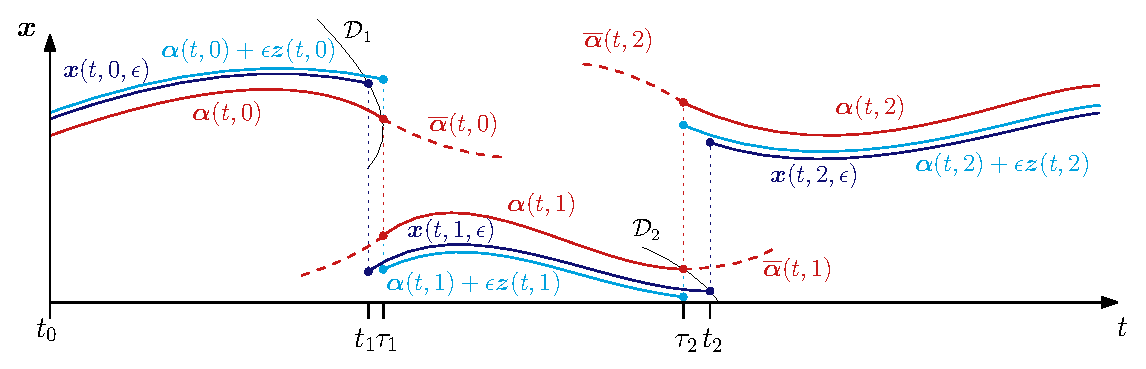
\includegraphics[width=.95\textwidth]{refspreadapprox.eps}\caption{The first order approximation $\alphab + \epsilon\zb$ (cyan) generated by the LTTHS is illustrated besides the perturbed trajectory $\xb$ (blue) and the nominal trajectory $\alphab$ (red). Note that the event times of the approximation are the same as those of the nominal trajectory.} \label{fig:3refspreadapprox}
\end{figure}

\section{Summary}
In this chapter, a linear first-order approximation of the NSITHS is presented. The NSITHS is formally defined, which is a framework suitable for the dynamics defined in Chapter~\ref{ch:model}. Perturbations in the initial condition and input curve are introduced into this system, resulting in perturbed trajectories of which the event times differ from the nominal event times, and are not known beforehand. This mismatch in event time leads to a behavior called peaking. Reference spreading is then presented to eliminate peaking behavior. After posing assumptions on continuity, transversality and the reference trajectory, a sensitivity analysis is performed. The sensitivity analysis leads to an LTTHS describing the tracking error dynamics, which is used to generate a first order approximation of the perturbed state. Under the presumption that a proof exists that uniform asymptotic stability of the LTTHS implies local asymptotic stability of the NSITHS, conventional stability analysis tools can be used to evaluate tracking of the nominal reference trajectory.


%% new chapter %%
\cleartooddpage
\chapter{Tracking for Hybrid Systems: Simultaneous State-and-Input-Triggered Events}\label{ch:simult}
The analysis presented in Chapter~\ref{ch:order} will be extended to be suitable for trajectories with simultaneous guard activations in this chapter. Simultaneous guard activations are activations where a trajectory triggers two or more guard functions at the same time-instant. Take for example a box with two contact points, where the contacts are closed at the same time. When perturbations are introduced in these trajectories, the simultaneity of the event can be lost. Also, the order of activations can change depending on the perturbation. The box can first impact one contact point and then at the other, or the other way around. This complicates the definition of the first-order approximation. In this chapter, a novel notation from \cite{Rijnen2018} will be presented to describe trajectories with simultaneous guard functions. Reference spreading is applied to trajectories with simultaneous events, which is used as a basis to define a positively homogeneous jump gain which approximates the jump behavior of the perturbed trajectory. The positively homogeneous jump gain defines the \textit{positively homogeneous time-triggered hybrid system} (PTTHS). This chapter extends the work presented in \cite{Rijnen2018}, making the approximation suitable for trajectories with input-dependent guard functions, and therefore mechanical systems experiencing dry friction and releasing motions.

\section{Simultaneous guard-activation}\label{sec:simguards}
To be able to perform the sensitivity analysis presented in Chapter~\ref{ch:order} for trajectories with simultaneous guard activations, some adjustments need to be made to the notation. In this section, a new notation \cite{Rijnen2018} is presented, namely: the event character, micro- and macro-events, multiscale hybrid time, guard function index, mode descriptor, phantom segments, and historical notation. After this, reference spreading for simultaneous guard-activations is discussed.

\subsection{Adopted notation}\label{sec:4not}
In a simultaneous event, more than one guard function is activated in one event. In Figure~\ref{fig:4simulexample}, an example of a simultaneous activation is illustrated. The ante-event reference trajectory, $\alphab(t,0)$, activates two guard functions, $\gamma_1$ and $\gamma_2$. The number of guard functions that are activated in a single nominal event is called the \textit{event character}. In the example in Figure~\ref{fig:4simulexample}, the event character $c = 2$.

\begin{figure}[h]
\centering
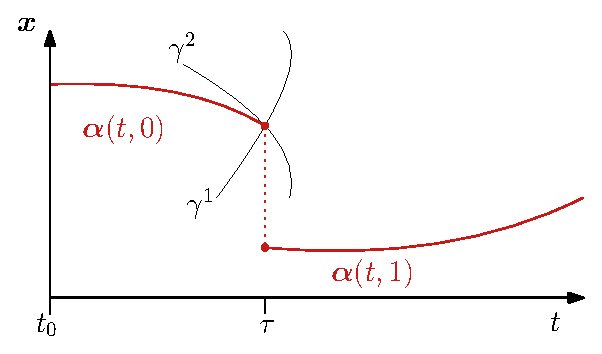
\includegraphics[width=.45\textwidth]{simulexample.eps}\caption{An illustration of a trajectory with a simultaneous event. At $t=\tau$, the trajectory activates two guard functions, $\gamma_1$ and $\gamma_2$.} \label{fig:4simulexample}
\end{figure}

When perturbations are introduced in an event with simultaneous activations, the number of events the system undergoes can change. Instead of a simultaneous activation of $c$ guards, the guards can be activated in rapid succession. These events that are the result of loss of simultaneity are called \textit{micro-events}, where several micro-events form one \textit{macro event}. Micro-events will generate extra segments in the state trajectory in comparison to the reference trajectory. To keep track of these segments, \textit{multiscale hybrid time} is introduced. Multiscale hybrid time is denoted by $(t,i,k)$, where $t$ is regular time, $i$ the macro-event counter, and $k$ the micro-event counter. The micro-event counter $k$ is incremented everytime an event occurs, except when a macro event is completed by reaching the nominal post-event mode. The micro-event counter $k$ is then reset to zero, and the macro-event counter $i$ is incremented. One can now write $\xb(t,i,k)$ to make a distinction between all the segments that are generated as a result of loss of simultaneity. Multiscale hybrid time is directly related to the regular hybrid time, according to
\begin{align}
j(i,k) = k + \sum_{I=1}^{i}l_I,
\end{align}
with $l_I$ the number of micro-events in macro-event $I$. The perturbed event times of micro-events are denoted by $t^k_i$, i.e., the event time of the $k^{\text{th}}$ micro-event of macro-event $i$. A set of guard function indexes $\eta$ is introduced to identify the several guard functions that are involved with an event. The index set of inactive guard functions is defined as
\begin{align}
\eta = 2^{\nu},\quad\text{with }\nu\in\{0,1,...,c_i\}.
\end{align}
$\eta$ is written in the binary numeral system for a more intuitive notation of the different guard functions. The inactive guard functions can then be denoted as $\gamma^\eta$. Note that
\begin{align}
\gamma^\eta = \gamma^\eta(\cdot,i,k),
\end{align}
meaning that the guard functions not only change with macro-events, but also with micro-events. While these counters are left out for readability, the reader should be aware that $\gamma^\eta$ can be different for each macro and micro-event. The modes that the system is in, is indicated using the \textit{mode descriptor} $s^k_i$. The mode descriptor $s^k_i$ is associated to event $i$, similar to $\tau_i$. The reader should be aware of the distinction between the event $i$ and the hybrid time $i$. The hybrid time $i$ indicates a segment of flow, whereas the event $i$ indicates a point. The micro-segments associated to macro-event $i$ can be described using
\begin{align}
\ls^{s^k_i}\xb(t) = \xb(t,i-1,k),
\end{align}
with $s^k_i$ the mode of the $k^{\text{th}}$ micro-event associated to macro-event $i$. When the considered macro-event is known from context, the macro-counter $i$ can be dropped to simplify the notation. From here on, we will write the mode descriptor as $s^k$. Similar to $\eta$, the mode descriptor is written in the binary numeral system. This binary numeral system is used as follows. When there is an event with character $c = 4$, four guard functions can be activated. When the mode of the system is $s^k = 1010$, this means that two guard functions remain inactive. Namely, the guard functions with index $\eta = \{0100,0001\}$. The mode descriptor now intuitively shows which guard functions are inactive, as the zeros in the mode descriptor denote the inactive guard function indexes. The index of the guard function that is activated during event $k$ is denoted by $\eta_k$.

We will illustrate the adopted notation in an example. Let us consider a transition, depicted in Figure~\ref{fig:4simulpert}, with event character $c = 2$, and guard functions $\gamma^{10}$ and $\gamma^{01}$. The system's state evolution begins in mode $s^0 = 00$, where $\gamma^{10},\gamma^{01}>0$. When the state activates one of the guard functions, in this case $\gamma^{01}=0$, the next mode becomes $s^1 = 01$. When the other guard function is activated as well, $\gamma^{10} = 0$, the system completes its macro-event with $s^2 = 11$. Note that the guard function can change when the system is in another mode, i.e., the guard function $\gamma^{10}$ defined in $s^0$ is different from the guard function $\gamma^{10}$ defined in $s^1$.

\begin{figure}[h]
\centering
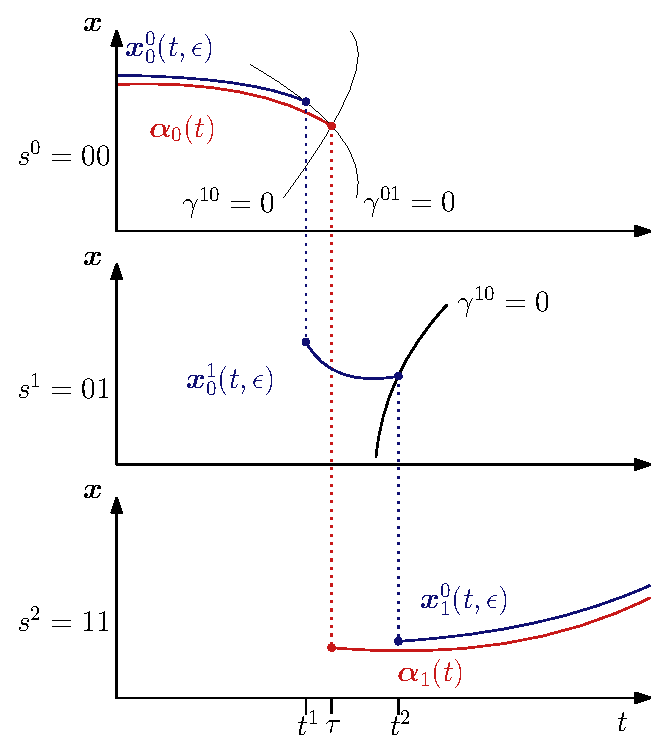
\includegraphics[width=.52\textwidth]{simulpert.eps}\caption{A reference trajectory going through a simultaneous event and a state trajectory experiencing loss of simultaneity. Where the reference trajectory activates $\gamma^{10}$ and $\gamma^{01}$ simultaneously, the state trajectory first activates $\gamma^{01}$ at $t=t^1$, flows for $t\in [t^1_1,t^2_1]$, and then activates $\gamma^{10}$ at $t=t^2$.}\label{fig:4simulpert}
\end{figure}

Depending on the perturbation, several mode sequences can achieve the expected nominal end mode when simultaneity is lost. The different mode sequences can generate a different post-event state, because of the flow phases in between the micro-events. Therefore, it is useful to be able to indicate an entire mode sequence with one symbol. We call this notation the \textit{historical notation}. We define the sequence for macro-event $i$ as 
\begin{align}
S^k_i = s^k_i\leftarrow s^{k-1}_i\leftarrow ... \leftarrow s^0_i,
\end{align}
where $s^0_i = 00...0$ with length $c_i$. Again, the macro-counter $i$ can be left out for convenience. A growing mode sequence is a sequence of micro-events, where at eacht micro-event another guard function is activated and no guard functions deactivated. We can now define $\ls^{S^k}\xb(t)$ as $\ls^{s^k}\xb(t)$ that is a result of the growing sequence $S^k$. The jump maps that are applied during such a sequence are given by
\begin{align}
\ls^{p}\xb = \ls^{p\leftarrow a}\gb(\ls^{a}\xb,\ls^{a}\ub,t),
\end{align}
where $p$ represents the post-event mode descriptor, and $a$ the ante-event mode descriptor. For example, the state jump from $s^k$ to $s^{k+1}$ is given by $\ls^{s^{k+1}}\xb = \ls^{s^{k+1}\leftarrow s^k}\gb(\ls^{s^k}\xb,\ls^{s^k}\ub,t)$. Sequences with a particular order of events can also be expressed as
\begin{align}
\ls^{\nu_k \nu_{k-1}...\nu_{1}}S^k = s^k \leftarrow s^{k-1} \leftarrow ... \leftarrow s^0,
\end{align}
where all mode descriptor entries are defined as $s^{\kappa} = s^{\kappa-1} + \eta_{\kappa}$, with $\eta_{\kappa} = 2^{\nu_{\kappa}-1}$ and $\kappa = \{1,2,...,k\}$. For a simultaneous activation during a micro-event, the participating guard functions are placed within brackets. For example, for a character-4 ($c = 4$) growing sequence, we write 
\begin{align}
\ls^{23(14)}S^3 = 1111 \leftarrow 1101 \leftarrow 1001 \leftarrow 0000.
\end{align}
\nomenclature[G]{$\kappa$}{Historical notation counter}%
Now that the notation for trajectories with simultaneous guard activations is in place, reference spreading for such activations is presented in the next section.

\subsection{Reference-spreading for simultaneous events}
For trajectories with simultaneous activations, the perturbed state can experience more events than the reference trajectory. The perturbed state will enter micro-modes and micro-segments, which are not seen in the reference trajectory. To be able to define a physically realistic comparison between the reference trajectory and the state trajectory, the reference trajectory needs to be adjusted accordingly. This is done in the form of \textit{nominal phantom modes} and \textit{nominal phantom segments}. Phantom modes are modes defined in the reference trajectory, that do not physically exist. Definition of these modes requires a property of the state jumps that we term associativity.
\begin{myass}[Jump map associativity]\label{ass:associativity}
We assume that the jump map $\ls^{p\leftarrow a}\gb(\ls^{a}\xb,\ls^{a}\ub,t)$ is associative, meaning that taking an arbitrary growing sequence $s^k\leftarrow s^{k-1} \leftarrow ... \leftarrow s^0$, where $p = s^k$ and $a = s^0$, it holds that
\begin{align}
\ls^{p}\xb = \left(\ls^{p\leftarrow s^{k-1}}\gb \circ \ls^{s^{k-1} \leftarrow s^{k-2}}\gb \circ \cdots \circ \ls^{s^1 \leftarrow a}\gb \right).
\end{align}
Intuitively, this means that the simultaneous jump gain from $a$ to $p$ can be described with a sequence of jumps evaluated at the same time instant.
\end{myass}
Using Assumption~\ref{ass:associativity}, the phantom modes can be defined. All micro-modes, which the state can enter as a result of loss of simultaneity, are defined in the nominal trajectory. These modes are called the phantom modes in the nominal trajectory. The initial states associated to these modes are found by applying the corresponding jump maps $\ls^{p\leftarrow a}\gb$ to the nominal ante-event state,
\begin{align}
\ls^{s_i^1}\alphab =&\ \ls^{s_i^1\leftarrow s_i^0}\gb(\ls^{s_i^0}\alphab,\ls^{s_i^0}\mub,\tau_i)\nonumber\\
&\vdots\label{eq:4phantomini}\\
\ls^{s_i^{k}}\alphab =&\ \ls^{s_i^k\leftarrow s_i^{k-1}}\gb(\ls^{s_i^{k-1}}\alphab,\ls^{s_i^{k-1}}\mub,\tau_i),\nonumber
\end{align}
resulting in a reference trajectory that goes through the same modes as the state trajectory. The feedforward term that defines the phantom modes can be chosen from two options. We define \textit{withdrawing phantom modes} and \textit{pushing phantom modes}, which are defined by the feedforwards
\begin{equation}
\ls^{S^k_i}_{\nearrow}\bar{\mub}(t) := \left\lbrace\begin{array}{ll}
\bar{\mub}_{i-1}(t), & k = 0\\
\bar{\mub}_i(t), & k \neq 0
\end{array},\right.
\end{equation}
and
\begin{equation}
\ls^{S^k_i}_{\searrow}\bar{\mub}(t) := \left\lbrace\begin{array}{ll}
\bar{\mub}_{i-1}(t), & k \neq l_i\\
\bar{\mub}_i(t), & k = l_i
\end{array},\right.\label{eq:4phantominp}
\end{equation}
\nomenclature[R]{$l_i$}{Number micro-events in macro-event $i$}%
where $\nearrow$ indicates a withdrawing feedforward and $\searrow$ indicates a pushing feedforward, and $l_i$ is the number of micro-events associated with macro-event $i$. For each event it should be specified whether a withdrawing or pushing phantom mode is used. 

Since the events of the state trajectory happen at different time-instant than the events in the reference trajectory, the phantom modes should be extended similarly as in Section~\ref{ch:order}. 
Using the initial states $\ls^{S_i^{k}}\alphab$ defined in \eqref{eq:4phantomini} and inputs $\ls^{S^k_i}\bar{\mub}$ defined in \eqref{eq:4phantominp}, the vector field $\ls^{s^k_i}\fb$ can be integrated forward and backward to find the (pushing or withdrawing) phantom segments corresponding to the phantom modes. These phantom modes and segments are illustrated in Figure~\ref{fig:4simulmicro}, where $\ls^{s_0^1}\bar{\alphab}(t),\ls^{s_1^1}\bar{\alphab}(t),\ls^{s_1^2}\bar{\alphab}(t)$ are examples of phantom segments.
\begin{figure}[h]
\centering
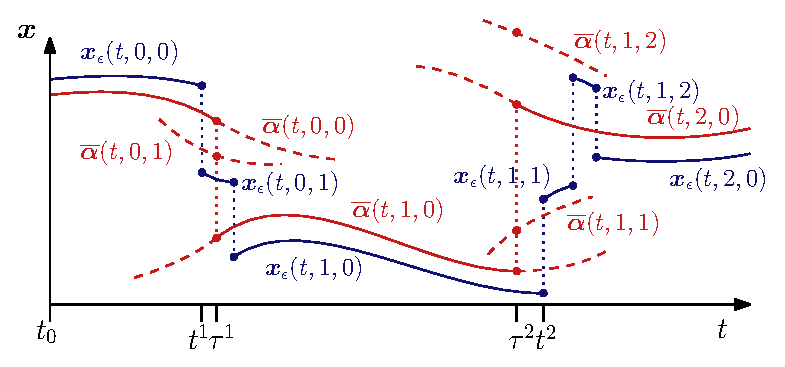
\includegraphics[width=.9\textwidth]{simulmicro.eps}\caption{The state evolution of the reference trajectory and state trajectory. Phantom segments are added to the reference trajectory, to which the micro-segments of the state trajectory can be compared.}\label{fig:4simulmicro}
\end{figure}

\nomenclature[R]{$i$}{The macro-event counter}%
\nomenclature[R]{$k$}{The micro-event counter}%
\nomenclature[R]{$c_i$}{The event-character of macro-event $i$}%
\nomenclature[R]{$l_i$}{The amount of simultaneous activations of macro-event $i$}%
\nomenclature[R]{$s^k_i$}{The event-mode descriptor of macro-event $i$ and micro-event $k$}%
\nomenclature[r]{$S^k_i$}{The historical notation of macro-event $i$ from micro-event $0$ up to $k$}%
\nomenclature[G]{$\eta$}{The set of indexes of inactive guards}%
\nomenclature[R]{$t_i^k$}{The perturbed event time of micro-event $k$ in macro-event $i$}%

\section{First-order approximation for trajectories with simultaneous guard-activation}
\textbf{INTRO}
\subsection{Sensitivity analysis for simultaneous guard-activation}
\textbf{CONTINUE HERE}

Now the sensitivity analysis for a trajectory with simultaneous events is presented. Similar to the sensitivity analysis for trajectories with isolated events, the continuous macro-segments ($k=0$) of the state can be approximated using
\begin{align}
\xb_i(\epsilon) = \bar{\alphab}_i + \epsilon\bar{\zb}_i + o(\epsilon),
\end{align}
where $\zb_i$ satisfies
\begin{align}
\dot{\zb}_i = \Ab_i(t)\zb_i +\Bb_i(t)\vb_i,\quad i\in \dom\alphab
\end{align}
with
\begin{align}
\Ab_i(t) &= D_1\fb_i(\alphab_i,\mub_i,t),\\
\Bb_i(t) &= D_2\fb_i(\alphab_i,\mub_i,t).
\end{align}
Now we derive a first order approximation of the jump map of a simultaneous event with character $c_i = 2$. A more thorough description of this derivation can be found in Appendix~\ref{app:multjumps}. In this chapter, the macro-counter $i$ is left out of the derivation for readability. The jump map that describes micro-event $k+1$ is given by
\begin{align}
\ls^{s^{k+1}}\xb_\epsilon(t^{k+1}) = \ls^{s^{k+1}\leftarrow s^k}\gb(\ls^{s^{k}}\xb_\epsilon(t^{k+1}),\ls^{s^{k}}\ub_\epsilon(t^{k+1}),t^{k+1}),\label{eq:4xe012}
\end{align}
with
\begin{align}
\ls^{s^{k}}\xb_\epsilon(t^{k+1}) = \int_{t^{k}}^{t^{k+1}}\left[\ls^{s^{k}}\fb\left(\ls^{s^{k}}\xb_\epsilon(t),\ls^{s^{k}}\ub_\epsilon(t),t\right)\right]dt + \ls^{s^{k}\leftarrow s^{k-1}}\gb(\ls^{s^{k-1}}\xb_\epsilon(t^{k}),\ls^{s^{k-1}}\ub_\epsilon(t^{k}),t^{k}).\label{eq:4xe01}
\end{align}
Here the subscript $(\cdot)_\epsilon$ indicates that the variable is dependent on $\epsilon$, the left superscript $\ls^{s^k}(\cdot)$ indicates that the variable is in micro-segment $k$, and $t^k$ represents the event-time of micro-event $k$. Now we expand the right-hand side of \eqref{eq:4xe012} with respect to $\epsilon$, to find
\begin{align}
\ls^{s^{k+1}}\xb_\epsilon(t^{k+1}) = \ls^{s^{k+1}}\alphab(\tau) + \epsilon\left.\frac{\partial}{\partial\epsilon}\ls^{s^{k+1}\leftarrow s^k}\gb\right|_{\epsilon=0} + o(\epsilon),\label{eq:4xe012exp}
\end{align}
where
\begin{multline}
\left.\frac{\partial}{\partial\epsilon}\ls^{s^{k+1}\leftarrow s^k}\gb\right|_{\epsilon=0} = D_1\ls^{s^{k+1}\leftarrow s^k}\gb\cdot\left(\ls^{s^{k}}\fb(\Delta^{k+1}-\Delta^{k}) + D_1\ls^{s^{k}\leftarrow s^{k-1}}\gb\cdot\left(\ls^{s^{k-1}}\zb+\ls^{s^{k-1}}\fb\Delta^{k}\right)\right. \\ \left.+ D_2\ls^{s^{k}\leftarrow s^{k-1}}\gb\cdot\left(\ls^{s^{k-1}}\vb+\ls^{s^{k-1}}\dot{\mub}\Delta^{k}\right) + D_3\ls^{s^{k}\leftarrow s^{k-1}}\gb\cdot\Delta^{k}\right)+D_3\ls^{s^{k+1}}\gb\cdot\Delta^{k+1}. \label{eq:4dg1de}
\end{multline}
Now, by expanding $\ls^{s^{k+1}}\xb_\epsilon(t^{k+1})$ with respect to $\epsilon$, we find
\begin{align}
\ls^{s^{k+1}}\xb_\epsilon(t^{k+1}) &= \ls^{s^{k+1}}\alphab(t^{k+1})+\epsilon\ ^{s^{k+1}}\zb(t^{k+1}) + o(\epsilon),\\
&= \ls^{s^{k+1}}\alphab(\tau) + \epsilon\ ^{s^{k+1}}\dot{\alphab}(\tau)\Delta^{k+1} + \epsilon\ ^{s^{k+1}}\zb(\tau) + o(\epsilon).\label{eq:4xexp}
\end{align}
Using \eqref{eq:4xe012exp} and \eqref{eq:4xexp}, an expression for $\ls^{s^{k+1}}\zb(\tau)$ is found, which is
\begin{multline}
\ls^{s^{k+1}}\zb(\tau) = D_1\ls^{s^{k+1}}\gb\cdot\ls^{s^{k}}\fb\Delta^{k+1} - D_1\ls^{s^{k+1}}\gb\cdot\ls^{s^{k+1}}\fb\Delta^{k} + D_1\ls^{s^{k+1}}\gb\cdot\left[D_1\ls^{s^{k+1}}\gb\cdot\left(\ls^{s^{k-1}}\zb+\ls^{s^{k-1}}\fb\Delta^{k}\right)\right.\\
\left.+D_2\ls^{s^{k}}\gb\cdot\left(\ls^{s^{k-1}}\vb+\ls^{s^{k-1}}\dot{\mub}\Delta^{k}\right)+D_3\ls^{s^{k}}\gb\cdot\Delta^{k}\right] + \left(D_3\ls^{s^{k+1}}\gb^{k} - \ls^{s^{k+1}}\fb\right)\Delta^{k+1},\label{eq:4ztau}
\end{multline}
which can be rewritten to 
\begin{multline}
\ls^{s^{k+1}}\zb(\tau) = \left(\frac{\ls^{s^{k+1}}\fb - D_1\ls^{s^{k+1}}\gb\cdot\ls^{s^{k}}\fb  - D_2\ls^{s^{k+1}}\gb\cdot\ls^{s^{k}}\dot{\mub} - D_3\ls^{s^{k+1}}\gb}{\ls^{s^{k+1}}\dot{\gamma}}D_1\ls^{s^{k+1}}\gamma + D_1\ls^{s^{k+1}}\gb\right)\Gb^{k}\ ^{s^{k-1}}\zb\\
+ \left(\frac{\ls^{s^{k+1}}\fb - D_1\ls^{s^{k+1}}\gb\cdot\ls^{s^{k}}\fb - D_2\ls^{s^{k+1}}\gb\cdot\ls^{s^{k}}\dot{\mub} - D_3\ls^{s^{k+1}}\gb}{\ls^{s^{k+1}}\dot{\gamma}}D_1\ls^{s^{k+1}}\gamma + D_1\ls^{s^{k+1}}\gb\right)\Jb^{k}\ ^{s^{k-1}}\vb\\
+ \left(\frac{\ls^{s^{k+1}}\fb-D_1\ls^{s^{k+1}}\gb\cdot\ls^{s^{k}}\fb - D_2\ls^{s^{k+1}}\gb\cdot\ls^{s^{k}}\dot{\mub} - D_3\ls^{s^{k+1}}\gb}{\ls^{s^{k+1}}\dot{\gamma}}D_2\ls^{s^{k+1}}\gamma\right)\ls^{s^{k}}\vb,
\end{multline}
which is equal to
\begin{align}
&\ls^{s^{k+1}}\zb(\tau) = \Gb^{k+1}\Gb^k\ ^{s^{k-1}}\zb + \Gb^{k+1}\Jb^{k}\ ^{s^{k-1}}\vb + \Jb^{k+1}\ ^{s^{k}}\vb.\label{eq:4zkplusfinal}
\end{align}
For brevity, the derivation has been reduced to essential equations. For a more complete derivation, consult Appendix~\ref{app:multjumps}. Note that \eqref{eq:4zkplusfinal} is also found by taking the first order approximation of two single jumps
\begin{align}
\ls^{s^{k}}\zb(\tau) &= \Gb^k\ ^{s^{k-1}}\zb + \Jb^{k}\ ^{s^{k-1}}\vb,\\
\ls^{s^{k+1}}\zb(\tau) &= \Gb^{k+1}\ ^{s^{k}}\zb + \Jb^{k+1}\ ^{s^{k}}\vb,
\end{align}
and substituting the one into the other. This implies that the first-order approximation of the post-impact state of two simultaneous jumps at $\tau$ can be found by evaluating the two jumps separately. For an arbitrary number of micro-events $k$, the first-order approximation of the post-event state can be found to be
\begin{align}
\ls^{S^k}\zb(\tau) = \ls^{s^k\leftarrow s^0}\Gb\ ^{s^0}\zb(\tau) + \sum_{\iota=0}^{k-1}\left(\ls^{s^{k}\leftarrow s^{\iota+1}}\Gb\ ^{s^{\iota+1}\leftarrow s^{\iota}}\Jb\ ^{s^{\iota}}\vb(\tau)\right),\label{eq:4ljumps}
\end{align}
where $\ls^{p\leftarrow a}\Gb$ and $\ls^{p\leftarrow a}\Jb$ are given by
\begin{align}
\ls^{p\leftarrow a}\Gb &:= \ls^{p}\Gb\ ^{p-1}\Gb\cdots\ls^{a}\Gb,\\
\ls^{p\leftarrow a}\Jb &:= \ls^{p}\Jb\ ^{p-1}\Jb\cdots\ls^{a}\Jb,
\end{align}
for a sequence $p\leftarrow p-1 \leftarrow \cdots \leftarrow a$. When $\vb$ is considered a feedback term and it is turned off when the first micro-event is detected, the first-order approximation of the post-event can be simplified to
\begin{align}
\ls^{S^k}\zb(\tau) &= \ls^{S^k}\Lb \begin{bmatrix}
\ls^{s^0}\zb(\tau) \\ \ls^{s^0}\vb(\tau)
\end{bmatrix}, \text{ with }\ls^{S^k}\Lb = \begin{bmatrix}
\ls^{S^k}\Gb & \ls^{S^{k\leftarrow 1}}\Gb\ls^{S^{1\leftarrow 0}}\Jb
\end{bmatrix},\label{eq:4ljumpssimp}
\end{align}
since only the ante-event feedback term will be non-zero. The jump gain defined in \eqref{eq:4ljumpssimp} is defined for a particular order of guard-activations. Note that the description of a jump gain for a micro-event where feedback is non-zero is more extensive than the jump gain given in \eqref{eq:4ljumpssimp}. However, since in this work only situations with zero feedback during micro-event are considered, the jump gain in \eqref{eq:4ljumpssimp} is used from here on to define $\ls^{S^k}\Lb$.

\subsection{The positively homogeneous jump gain}
As mentioned in Section~\ref{sec:simguards}, an event with simultaneous guard activation will experience loss of simultaneity when perturbations are introduced. Due to the loss of simultaneity, the order of events is unknown. For that reason, one simultaneous event has several associated event sequences. For there to be a finite amount of possibilities of event sequences, all sequences should be growing. This assumption is now formally defined.

\begin{myass}[Growing mode sequences]\label{ass:unidirectional}
We assume, locally at each macro-event, that all considered mode sequences are growing, meaning that at each micro-event, one or more guard functions become active, without changing the status of any other guard functions. In other words, considering one macro-event, we assume that $s^0<s^1<...<s^l$, where $s^0= 00...0$ and $s^l = 11...1$, and $l$ is the number of micro-events in the considered macro-event.
\end{myass}

For example, when we consider a block with two contact points $\iota_1$ and $\iota_2$ executing a pushing motion towards a surface, with $s^0 = 00$ is both contact points open and $s^l = 11$ is both contact points in closed contact stick. Let us say we are in mode $s^1 = 10$, i.e. $\iota_1$ is in closed contact stick and $\iota_2$ still open. Now the system goes through the second micro-event by activating $\gamma^{01}_2$. Under Assumption~\ref{ass:unidirectional}, the event can not cause $\iota_1$ to release contact, i.e., $\Gamma_{\iota_1}^{\text{cl}\rightarrow\text{op}}>0$, $\Gamma_{\iota_1}^{\text{st}\rightarrow\text{sl}}>0$, $\gamma_{\iota_1}^{\text{cl}\rightarrow\text{op}}>0$ and $\gamma_{\iota_1}^{\text{st}\rightarrow\text{sl}}>0$ when solving the state reinitialization and mode selection presented in Section~\ref{sec:2discdyn}. Under Assumption~\ref{ass:unidirectional}, all mode sequences in a neighborhood of $\alphab,\mub$ will be growing and a finite number of jump gains are possible for a range of perturbations. Now an assumption on the association between guard functions and transitions is given. This assumption is necessary to prevent notation issues in the mode descriptor introduced in Section~\ref{sec:4not}.

\begin{myass}[Guard-transition association]\label{ass:guardtrans}
We assume that activation of the guard associated to contact point $\iota$ will result in a transition of only contact point $\iota$. With guard function $\gamma^{\eta_k}$ activated in mode $s^{k-1}$, the mode descriptor of the next mode satisfies $s^{k} = s^{k-1} + \eta_k$. Here $\eta_k$ is the index of the guard function that is activated during micro-event $k$.
\end{myass}

\begin{myremark}
Assumption~\ref{ass:guardtrans} is trivial for most guard functions. Because $\gamma^{\text{op}\rightarrow\text{cl}}_{\iota} = h_{n,\iota}(\qb)$ is defined on position level, under Assumption~\ref{ass:unidirectional} it will always be contact point $\iota$ that will change mode when $\gamma^{\text{op}\rightarrow\text{cl}}_{\iota}$ is activated. For guard functions defined on acceleration level, i.e.,
\begin{align}
\gamma^{\textnormal{st}\rightarrow\textnormal{sl}} &= \mu_\iota^2\lambda_{n,\iota} - \lambdab^T_{t,\iota}\lambdab_{t,\iota}\nonumber\\
\gamma^{\textnormal{cl}\rightarrow\textnormal{op}} &= \lambda_{n,\iota},\nonumber
\end{align}
the situation is different. The feasible post-event mode is determined by the post-event acceleration for these guard functions. It is therefore possible that a guard function is activated in mode $s^{k-1}$, but is inactive in mode $s^{k}$. Under Assumption~\ref{ass:guardtrans} this is not possible. Therefore a constraint is introduced on the post-event acceleration, which can be determined by the set of equations, called the mode selection in Section~\ref{sec:2discdyn},
\begin{align}
\ddot{\qb}^+ &= \Mb^{-1}\left[\Sb\ub^+ - \Cb + \Wb_{n}\lambdab^+_{n} + \Wb_{t}\lambdab^+_{t}\right], &  \nonumber\\
\wb^T_{n,\iota}\ddot{\qb}^+ + \dot{\wb}^T_{n,\iota}\dot{\qb}^+ &= 0, & \forall \iota\in\Ic_{\text{cl}},\nonumber\\
\lambdab^+_{t,\iota} + \mu\lambda^+_{n,\iota}\SgnSp(\Wb_{t,\iota}^T\dot{\qb}^+) &= 0, & \forall \iota\in\Ic_{\text{sl}},\nonumber\\
\Wb^T_{t,\iota}\ddot{\qb}^+ + \dot{\Wb}^T_{t,\iota}\dot{\qb}^+ &= 0. & \forall \iota\in\Ic_{\text{st}},\nonumber
\end{align}
From the mode selection we can conclude that the post-event acceleration $\ddot{\qb}$ is directly dependent on the post-event input $\ub^+$. Therefore, the post-event input $\ub^+$ should be chosen in such a way that Assumption~\ref{ass:guardtrans} is met.
\end{myremark}

Now a jump gain for a simultaneous event will be defined. This jump gain should consider all growing sequences that can take place for that range of perturbations. Therefore, a state-dependent matrix gain is defined, in the form of
\begin{align}
\ls^{p \leftarrow a}\Hb(\ls^{a}\zb(\tau),\ls^{a}\vb(\tau),\tau) = \left\lbrace\begin{array}{ll}
\Lb^1(\ls^{s^0}\zb,\ls^{s^0}\vb,\tau), & \text{if condition 1 is true},\\
\Lb^2(\ls^{s^0}\zb,\ls^{s^0}\vb,\tau), & \text{if condition 2 is true},\\
\vdots & \vdots\\
\Lb^{r}(\ls^{s^0}\zb,\ls^{s^0}\vb,\tau), & \text{if condition }r\text{ is true},
\end{array}\right.\label{eq:4Hgeneral}
\end{align}
where $\Lb$ is in the form of \eqref{eq:4ljumpssimp} and $r$ the number of possible mode sequences in a macro-event. We will now derive the jump maps and associated conditions in \eqref{eq:4Hgeneral} to make the expression explicit.

For a certain perturbation, only a single order of micro events is feasible. This order can be found by determining the perturbed jump time of all possible micro events, and selecting the micro event with the earliest impact time as the next event. Mathematically, this is written as
\begin{align}
s^{k+1} = \underset{s^{k+1}}{\argmin}\left(\ ^{s^{k+1} \leftarrow S^{k}}t_\epsilon\right).\label{eq:4argmin1}
\end{align}
The perturbed event-time of the next micro-event $\ ^{s^{k+1} \leftarrow S^{k}}t_\epsilon$ can be approximated using the first order approximation
\begin{align}
\ls^{s^{k+1} \leftarrow S^{k}}t_\epsilon = \tau + \epsilon\Delta^{k+1}.
\end{align}

Now, since $\tau$ and $\epsilon$ are equal for each impact time, we can rewrite \eqref{eq:4argmin1} to

\begin{align}
s^{k+1} = \underset{s^{k+1}}{\argmin}\left(\Delta^{k+1}\right),
\end{align}
which can be written as
\begin{align}
s^{k+1} = s^k + \underset{\eta^*}{\argmin}\left(-\frac{D_1\gamma^{\eta^*}(\ls^{s^k}\alphab,\ls^{s^k}\mub,\tau)\cdot\ls^{S^k}\zb + D_2\gamma^{\eta^*}(\ls^{s^k}\alphab,\ls^{s^k}\mub,\tau)\cdot\ls^{S^k}\vb}{\dot{\gamma}^{\eta^*}}\right),
\end{align}
with $\eta$ the set of guard identifiers that are still open and $\eta^*$ the indexes of the guard functions in $\eta$. Then
\begin{align}
\eta^{k+1} = \underset{\eta^*}{\argmin}\left(-\frac{D_1\gamma^{\eta^*}(\ls^{s^k}\alphab,\ls^{s^k}\mub,\tau)\cdot\ls^{S^k}\zb + D_2\gamma^{\eta^*}(\ls^{s^k}\alphab,\ls^{s^k}\mub,\tau)\cdot\ls^{S^k}\vb}{\dot{\gamma}^{\eta^*}}\right),\label{eq:4argmin2}
\end{align}
with $s^{k+1} = s^k + \eta^{k+1}$ and $\eta^{k+1}$ the index of the guard function the will be activated during event $k+1$. Finally, with
\begin{align}
\ls^{S^k}\ab &= -\frac{1}{\dot{\gamma}^{\eta^k}}D_1\gamma^{\eta^k}(\ls^{s^k}\alphab,\ls^{s^k}\mub,\tau),\\
\ls^{S^k}\bb &= -\frac{1}{\dot{\gamma}^{\eta^k}}D_2\gamma^{\eta^k}(\ls^{s^k}\alphab,\ls^{s^k}\mub,\tau),
\end{align}
\eqref{eq:4argmin2} can be rewritten as
\begin{align}
\eta^{k+1} = \underset{\eta^*}{\argmin}\left(\ls^{S^k}\ab^T\ls^{S^k}\zb +\ls^{S^k}\bb^T\ls^{S^k}\vb\right).
\end{align}
Now, by checking \eqref{eq:4argmin2} for every micro event, we know which jump gains we should take to substitute into \eqref{eq:4ljumps}.
For example a system with $c_i = 2$, $\ls^{s^1}\vb=\ls^{s^2}\vb=...=\ls^{s^l}\vb=0$, and with a macro event starting in $s^0 = 00$ and ending in $s^l = 11$, this gives 
\begin{align}
\ls^{11\leftarrow 00}\Hb(\ls^{s^0}\zb(\tau),\ls^{s^0}\vb(\tau),\tau) = \left\lbrace\begin{array}{ll}
\begin{bmatrix}\ls^{11\leftarrow 00}_{\ls^{(12)}S^1}\Gb, & \ls^{11\leftarrow 00}_{\ls^{(12)}S^1}\Jb\end{bmatrix}, & \text{if }(\text{I}),\\
\begin{bmatrix}\ls^{11\leftarrow 01}_{\ls^{12}S^2}\Gb \ls^{01\leftarrow 00}_{\ls^{2}S^1}\Gb, & \ls^{11\leftarrow 01}_{\ls^{12}S^2}\Gb \ls^{01\leftarrow 00}_{\ls^{2}S^1}\Jb\end{bmatrix}, & \text{if }(\text{II}),\\
\begin{bmatrix}\ls^{11\leftarrow 10}_{\ls^{12}S^2}\Gb \ls^{10\leftarrow 00}_{\ls^{2}S^1}\Gb, & \ls^{11\leftarrow 10}_{\ls^{12}S^2}\Gb \ls^{10\leftarrow 00}_{\ls^{2}S^1}\Jb\end{bmatrix}, & \text{if }(\text{III}),
\end{array}\right.\label{eq:4H2200}
\end{align}
with
\begin{align}
(\text{I})&:\ls^{^2 S^1}\ab^T\ls^{^2 S^1}\zb +\ls^{^2 S^1}\bb^T\ls^{^2 S^1}\vb = \ls^{^1 S^1}\ab^T\ls^{^1 S^1}\zb +\ls^{^1 S^1}\bb^T\ls^{^1 S^1}\vb,\nonumber\\
(\text{II})&:\ls^{^2 S^1}\ab^T\ls^{^2 S^1}\zb +\ls^{^2 S^1}\bb^T\ls^{^2 S^1}\vb > \ls^{^1 S^1}\ab^T\ls^{^1 S^1}\zb +\ls^{^1 S^1}\bb^T\ls^{^1 S^1}\vb,\label{eq:4conds}\\
(\text{III})&:\ls^{^2 S^1}\ab^T\ls^{^2 S^1}\zb +\ls^{^2 S^1}\bb^T\ls^{^2 S^1}\vb < \ls^{^1 S^1}\ab^T\ls^{^1 S^1}\zb +\ls^{^1 S^1}\bb^T\ls^{^1 S^1}\vb.\nonumber
\end{align}

The jump gain in \eqref{eq:4H2200} is called a positively homogeneous jump gain for character-2 events. Due to the behavior of the simultaneous events, the linearity property of the jump gain is lost. This is shown in Appendix~\ref{app:poshom}. Instead, the jump gain is positively homogeneous, which is now formally defined.
 
\begin{mydef}[Positive homogeneity]
Suppose that $\fb(\xb,\ub,t)$ is a continuously differentiable function. The function $\fb$ is called positively homogeneous of degree $k$, if 
\begin{align}
\fb(a\xb,a\ub,t) = a^k\fb(\xb,\ub,t),
\end{align}
for all $a>0$.
\end{mydef}

The conditions that decide which jump gain to use are illustrated in Figure~\ref{fig:4cone}. Since the conditions are linear in $\zb$ and $\vb$, they appear as lines in the state space of $\zb$ and $\vb$. When we introduce more conditions, we will find several cones that relate a certain jump gain to a $\zb,\vb$ pair. When we look at the vector $r(\zb,\vb)$ in Figure~\ref{fig:4cone}, it can be noticed that when $\rb$ is multiplied with a positive constant $a$, the same jump gain is applied. Therefore, the positively homogeneous jump gain \eqref{eq:4H2200} is positively homogeneous of order zero.

\begin{figure}[H]
\centering
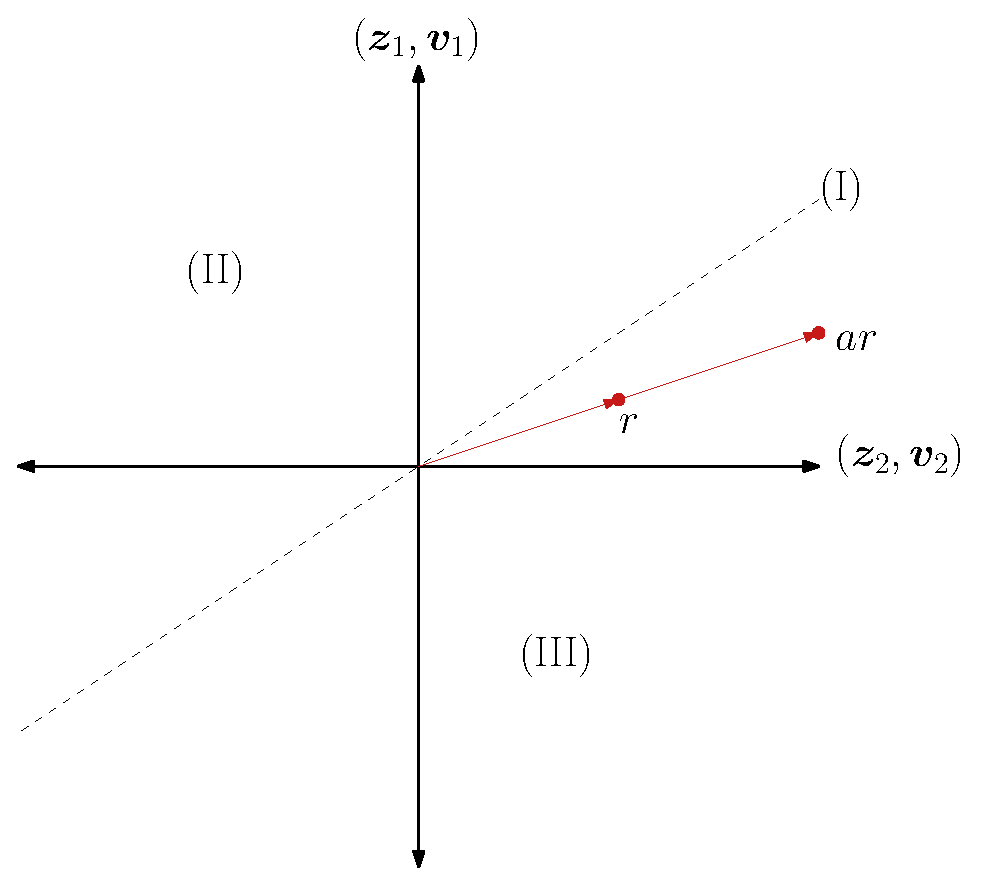
\includegraphics[width=.5\textwidth]{4cone.eps}\caption{An illustration of the positive homogeneity of order zero attribute of the positively homogeneous jump gain. The areas \textnormal{(I)}, \textnormal{(II)}, and \textnormal{(III)} coincide with the conditions in \eqref{eq:4conds}.}\label{fig:4cone}
\end{figure}

%\begin{figure}[h!]
%\centering
%\begin{subfigure}[b]{0.47\textwidth}   
%\centering 
%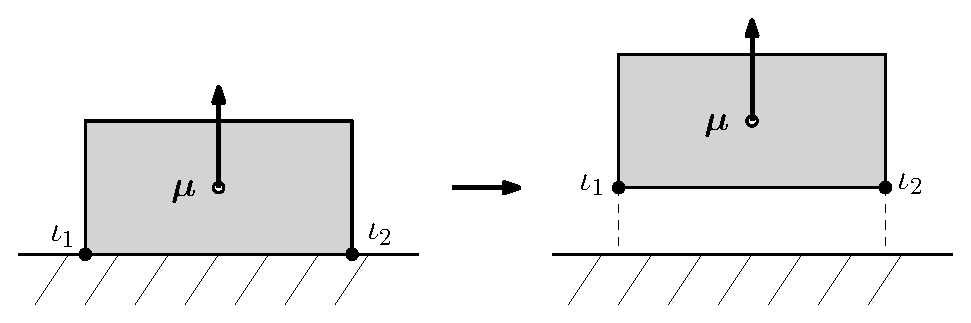
\includegraphics[width=\textwidth]{4example12.eps}
%\label{fig:4example1}\caption{The modes in the nominal trajectory.}
%\end{subfigure}
%\vskip\baselineskip
%\begin{subfigure}[b]{0.81\textwidth}   
%\centering 
%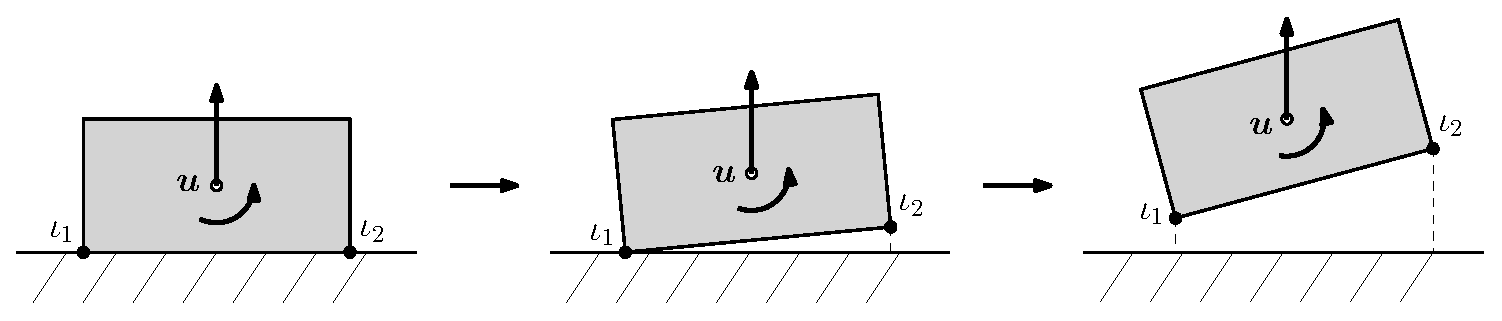
\includegraphics[width=\textwidth]{4example456.eps}
%\label{fig:4example4}\caption{The modes in a perturbed trajectory.}
%\end{subfigure}
%\vskip\baselineskip
%\begin{subfigure}[b]{\textwidth}   
%\centering 
%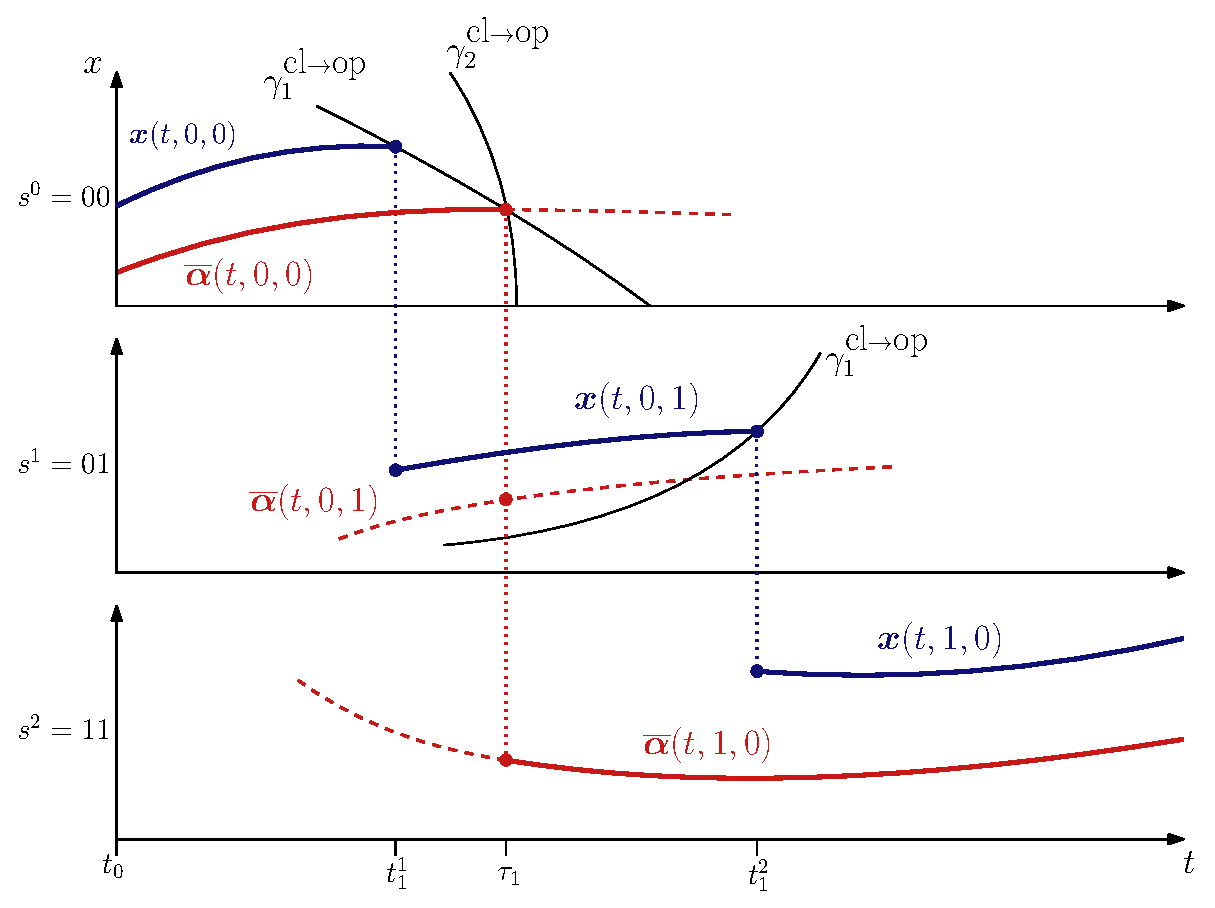
\includegraphics[width=.85\textwidth]{4exampletraj.eps}
%\label{fig:4exampletraj}
%\end{subfigure}
%\caption{The state evolution of the nominal and state trajectory is illustrated in this figure. }
%\label{fig:4example}
%\end{figure}

\subsection{The positively homogeneous time-triggered hybrid system}\label{def:4PTTHS}
\textbf{COMMENTS}
Now, with the positively homogeneous jump gain defined, the PTTHS can be defined. The PTTHS forms a first-order approximation of the NSITHS defined in Definition~\ref{def:3nsiths}. The proof that uniform asymptotic stability of the PTTHS does not yet exist for the NSITHS. However, similar to the relation between the LTTHS and NSITHS, we presume that a proof exists for the stability of the PTTHS implying local asymptotic stability of NSITHS. The PTTHS will jump at the same time as the nominal trajectory $\alphab$, and will also experience the same number of jumps. This means that a controller designed on the PTTHS will not act on micro-events. This is desired behavior, as the micro-events will likely happen too rapidly to control on. We now define the PTTHS formally, with the positively homogeneous jump gain being defined for a character-2 event ($c = 2$, with $a = 00$ and $p=11$) for brevity reasons.

\begin{mydef}[PTTHS]
The positively homogeneous time-triggered hybrid system associated with the NSITHS and the associative and transversal reference trajectory ($\alphab(t,i),\mub(t,i)$) is given by
\begin{align}
\dot{\zb}(t,i) &= \Ab(t,i)\zb(t,i) + \Bb(t,i)\vb(t,i), &(t,i) \in \dom\ \alphab,\\
\ls^{p}\zb &= \ls^{p\leftarrow a}\Hb(\ls^a\zb,\ls^a\vb,t)\begin{bmatrix} \ls^a\zb \\ \ls^a\vb\end{bmatrix}, &(t,i) \in \eve\ \alphab,
\end{align}
where $\ls^{p\leftarrow a}\Hb(\ls^a\zb,\ls^a\vb,t)$ is the positively homogeneous jump gain of order zero,
\begin{align}
A(t,i) &= D_1\fb(\alphab(t,i),\mub(t,i),t,i),\\
B(t,i) &= D_2\fb(\alphab(t,i),\mub(t,i),t,i),\\
\ls^{a}\zb & = \zb(t,i),\\
\ls^{a}\vb & = \vb(t,i),\\
\ls^{p}\zb & = \zb(t,i+1),
\end{align}
with $a = s_i^0 = 00...0$ and $p = s_i^l = 11...1$ where $l$ is the amount of micro-events in the growing sequence $p\leftarrow...\leftarrow a$. The set $\dom\ \alphab$ and $\eve\ \alphab$ are defined as
\begin{align}
\dom\ \alphab &:= \bigcup_{i=0}^N[\tau_i,\tau_{i+1}]\times \{i\},\\
\eve\ \alphab &:= \bigcup_{i=1}^N\{\tau_i\}\times \{i-1\},
\end{align}
and $\tau_0 = t_0$. The positively homogeneous jump gain $\ls^{p\leftarrow a}\Hb$ for a character-2 event ($c=2$), with the macro-counter $i$ omitted for readability, is given by
\begin{align}
\ls^{11\leftarrow 00}\Hb(\ls^{s^0}\zb(\tau),\ls^{s^0}\vb(\tau),\tau) = \left\lbrace\begin{array}{ll}
\begin{bmatrix}\ls^{11\leftarrow 00}_{\ls^{(12)}S^1}\Gb, & \ls^{11\leftarrow 00}_{\ls^{(12)}S^1}\Jb\end{bmatrix}, & \text{if }(\textnormal{I}),\\
\begin{bmatrix}\ls^{11\leftarrow 01}_{\ls^{12}S^2}\Gb \ls^{01\leftarrow 00}_{\ls^{2}S^1}\Gb, & \ls^{11\leftarrow 01}_{\ls^{12}S^2}\Gb \ls^{01\leftarrow 00}_{\ls^{2}S^1}\Jb\end{bmatrix}, & \text{if }(\textnormal{II}),\\
\begin{bmatrix}\ls^{11\leftarrow 10}_{\ls^{12}S^2}\Gb \ls^{10\leftarrow 00}_{\ls^{2}S^1}\Gb, & \ls^{11\leftarrow 10}_{\ls^{12}S^2}\Gb \ls^{10\leftarrow 00}_{\ls^{2}S^1}\Jb\end{bmatrix}, & \text{if }(\textnormal{III}),
\end{array}\right.\label{eq:4PTTHS1}
\end{align}
with
\begin{align}
(\textnormal{I})&:\ls^{^2 S^1}\ab^T\ls^{^2 S^1}\zb +\ls^{^2 S^1}\bb^T\ls^{^2 S^1}\vb = \ls^{^1 S^1}\ab^T\ls^{^1 S^1}\zb +\ls^{^1 S^1}\bb^T\ls^{^1 S^1}\vb,\\
(\textnormal{II})&:\ls^{^2 S^1}\ab^T\ls^{^2 S^1}\zb +\ls^{^2 S^1}\bb^T\ls^{^2 S^1}\vb > \ls^{^1 S^1}\ab^T\ls^{^1 S^1}\zb +\ls^{^1 S^1}\bb^T\ls^{^1 S^1}\vb,\\
(\textnormal{III})&:\ls^{^2 S^1}\ab^T\ls^{^2 S^1}\zb +\ls^{^2 S^1}\bb^T\ls^{^2 S^1}\vb < \ls^{^1 S^1}\ab^T\ls^{^1 S^1}\zb +\ls^{^1 S^1}\bb^T\ls^{^1 S^1}\vb.\label{eq:4PTTHS2}
\end{align}
The jump gains $\ls^{s^+\leftarrow s^-}_{S^k}\Gb$ and $\ls^{s^+\leftarrow s^-}_{S^k}\Jb$ in \eqref{eq:4PTTHS1}, with $s^+ = s^k$ and $s^- = s^0$ and $S^k = s^k\leftarrow s^{k-1} \leftarrow \cdots \leftarrow s^0$, are given by
\begin{align}
\ls^{s^+\leftarrow s^-}_{S^k}\Gb &:= D_1\gb^- - \left(\dot{\gb}^- - \fb^+\right)\frac{D_1\gamma^-}{\dot{\gamma}^-},\\
\ls^{s^+\leftarrow s^-}_{S^k}\Jb &:= D_2\gb^- - \left(\dot{\gb}^- - \fb^+\right)\frac{D_2\gamma^-}{\dot{\gamma}^-},
\end{align}
and
\begin{align}
\fb^- &= \ls^{s^-}\fb\left(\ls^{S^-}\alphab(\tau),\ls^{S^-}_{\rightarrow}\mub(\tau),\tau\right),\\
\fb^+ &= \ls^{s^+}\fb\left(\ls^{S^+}\alphab(\tau),\ls^{S^+}_{\rightarrow}\mub(\tau),\tau\right),\\
\gb^- &= \ls^{s^+\leftarrow s^-}\gb\left(\ls^{S^-}\alphab(\tau),\ls^{S^-}_{\rightarrow}\mub(\tau),\tau\right),\\
\gamma^- &= \gamma^{\eta(s^+\leftarrow s^-)}\left(\ls^{S^-}\alphab(\tau),\ls^{S^-}_{\rightarrow}\mub(\tau),\tau\right),\\
\dot{\gb}^- &= D_1\gb^-\cdot \fb^- + D_2\gb^-\cdot \dot{\mub}^- + D_3\gb^-,\\
\dot{\gamma}^- &= D_1\gamma^-\cdot\dot{\alphab}(\tau) + D_2\gamma^-\cdot\dot{\mub}(\tau) + D_3\gamma^-,
\end{align}
where the $\rightarrow$ left subscript should be interpreted as $\searrow$ or $\nearrow$ to indicate whether the feedforward is pushing or withdrawing, respectively. $\gamma^{\eta(s^+\leftarrow s^-)}$ is the guard function that is activated during the transition $s^+\leftarrow s^-$. If the transition $s^+\leftarrow s^-$ is associated with multiple guard functions, one of the guard functions can be chosen, as it will have no effect on the jump gain. For example, during the transition $11\leftarrow 00$, $\gamma^{01}$ or $\gamma^{10}$ should be used for defined the jump gain. Finally, the vectors $\ls^{S^k}\ab^T$ and $\ls^{S^k}\bb^T$ in \eqref{eq:4PTTHS2} are given by
\begin{align}
\ls^{S^k}\ab &= -\frac{1}{\dot{\gamma}^{-}}D_1\gamma^{-},\\
\ls^{S^k}\bb &= -\frac{1}{\dot{\gamma}^{-}}D_2\gamma^{-}.
\end{align}
\end{mydef}

\nomenclature[R]{$\Hb$}{The positively homogeneous jump gain}%
\nomenclature[R]{$\zb$}{The state perturbation}%
\nomenclature[R]{$\vb$}{The input perturbation}%
\nomenclature[R]{$\Ab$}{Linear state matrix}%
\nomenclature[R]{$\Bb$}{Linear input matrix}%
\nomenclature[A]{PTTHS}{Positively homogeneous Time-Triggered Hybrid System}%

\section{Summary}
A first-order approximation for nonlinear state-and-input-triggered systems with input-dependent guard experiencing simultaneous impacts is presented. Simultaneous guard activations are introduced, and the adopted notation required to deal with such activations is presented and elaborated. Assumptions on the reference trajectory are presented, which reduce the complexity of the problem while maintaining practical usability. Then, reference spreading is extended to transitions with simultaneous events. After that, a sensitivity analysis is performed, to find a first-order approximation of the behavior of the behavior of the NSITHS near $\alphab,\mub$, where so-called loss of simultaneity occurs. A state-and-input dependent jump gain, called the positively homogeneous jump gain, is used to define the positively homogeneous time-triggered hybrid system. This positively homogeneous hybrid system is expected to be suitable for assessing the local asymptotic stability of a nonlinear state-and-input triggered hybrid system with simultaneous guard activations.
\end{document}